It has been shown that the \emph{HP} model is a NP hard problem, so it's very difficult to fold efficiently longer protein sequences.
We will now discuss the Rosenbluth sampling method \cite{PERM}, which involves drawing successive steps of a random walk only from among acceptable points, which are points previously not visited.

\subsection{Self-Repelling Chains}
In a random walk process on $\mathbb{G} = \mathbb{Z}^3$, each iteration consist in a step among one out of six equally likely directions.
An analogue result is valid for $\mathbb{G} = \mathbb{Z}^2$ where we can choose one out of four equally likely directions.
Our goal is to simulate the folding of a protein of length $k$ in the space $\mathbb{G}$ by doing a random walk of $k$ steps.
The first thing we can notice is that this cannot be a regular random walk process because the fold is not allowed to cross itself or back up on itself at any iteration.
The direct consequence is that each iteration of the random walk will have some constraints, e.g. all steps after the first one will have at least one forbidden direction (because they cannot back up).
At this point, we can define as \emph{Self-Avoiding Walk} (SAW) a lattice path that does not visit the same point more than once.
\begin{figure}[H]
    \centering
    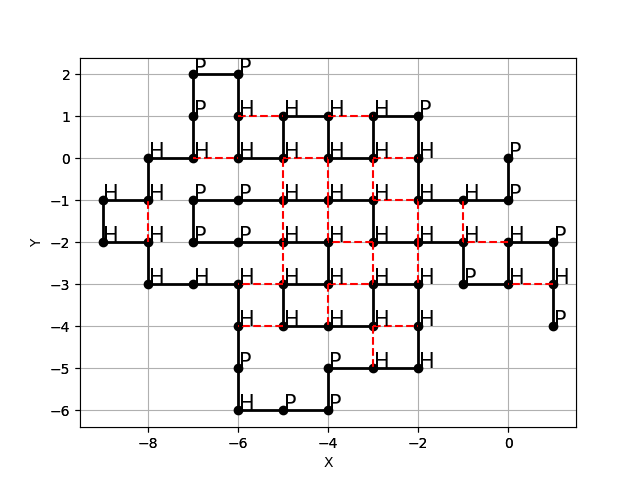
\includegraphics[width=.75\textwidth]{./img/src_example.png}
    \caption{\emph{Example of a self repelling chain starting from the origin of a square cubic lattice.
                    Each node represents an amino acid.
                    The red dashed lines represents the $H$-$H$ contacts.}}
    \label{fig:src_example}
\end{figure}
It is known that SAWs are fractals and their number on a given lattice will increase exponentially with the length \cite{madras1988pivot}.
However, there's a quite important difference between a ``true'' SAW and the problem we're interested in.
It has been proven \cite{trueSAW} that a SAW differentiates from a Self-Repelling Chain (polymer problem, see Fig. \ref{fig:src_example}) by a statistical point of view.
In fact, in an SRC, every possible configuration of the chain is equiprobable while this statement is not true for a SAW.
The result is that, since the statistics of the SRC is equivalent to the $n \to 0$ limit of an $O(n)$ symmetric $\phi^4$ field theory, the upper critical dimensionality for it turns out to be 4 vs 2 for a SAW.
We won't go deeper in this aspect because it is beyond the scope of this project.
The solution of an SRC is based on a \emph{constraint programming} approach, in which we try to solve a Constraint Satisfaction Problem like that.

\subsection{Estimate the number of folds}
For simplicity, let's assume that our SRC starts form the origin of our lattice.
At any iteration $m$ we will have only $w_m$ possible moves, where $w$ represents a sort of weight of our chain.
Let's call $W$ the weight of the whole fold: a fold of length $k$ will have a weight
\begin{equation*}
    W_k = \prod_{m=1}^k w_m
\end{equation*}
It is not excluded that at a certain step $m < k$ we may have no further possibilities for continuation: we then say that a \emph{non-extendable} fold of length $m$ has been formed.
Let's denote with $\mathcal{K}$ the set of all folds with length $m \leq k$.
Clearly $\mathcal{Z}_k \subset \mathcal{K}$.
We notice that the probability of picking a random fold $f_i \in \mathcal{K}$ of length $k$ is
\begin{equation*}
    \mathbb{P}\left(f_i \in \mathcal{Z}_k\right) = \prod_{j=1}^k \frac{1}{w_j} = \frac{1}{W_k}
\end{equation*}
Let's now denote with $n_y$ the number of folds $f_i$ for which $W\left(f_i\right) = y$ and the set of these elements $\mathcal{W}_y = \left\{f \in \mathcal{K} \ | \ W\left(f_i\right) = y\right\}$.
Then, for the law of large numbers
\begin{equation*}
    \frac{n_s}{n} \approx \mathbb{P}\left(\mathcal{W}_y\right)
\end{equation*}
In the same way we can notice that
\begin{equation*}
    \left\langle W \right\rangle = \frac{1}{n} \sum_{i=1}^n W\left(f_i\right) \approx \sum_f \mathbb{P}\left(f\right)W\left(f\right) = \sum_{f \in \mathcal{Z}_k} 1 = \left\lvert \mathcal{Z}_k \right\rvert
\end{equation*}
So we've found an estimator for the number of folds
\begin{equation}
    \hat{\mathcal{Z}_k} = \left\langle W \right\rangle \approx \left\lvert \mathcal{Z}_k \right\rvert
\end{equation}
Notice that this estimator does not give the number of \emph{unique} folds.
Using the \emph{batch mean method} we are also able to estimate the variance of our estimator.
Subdividing the sequence of weights $W\left(f_1\right),\ldots,W\left(f_n\right)$ into $j$ blocks of length $l$ each, so $n = jl$.
Defining the mean of the $b$-th block as
\begin{equation*}
    \mu_b = \frac{1}{l} \sum_{i = (b-1)l + 1}^{bl} W\left(f_i\right)
\end{equation*}
we can define our estimator for the variance as
\begin{equation}
    \hat{\sigma} = \sqrt{\frac{1}{j} \sum_{b = 1}^j \left(\mu_b - \left\langle W \right\rangle\right)^2}
\end{equation}